%!TEX root = ../../main.tex

\subsection{KarControl BDD}
\systemBDD{0.82}{KarControl}

\subsubsection{KarGruppe}
KarGruppe er den overordnede betegnelse for et vandkar med tilførende pH-værdi og gødningskoncentration. KarGruppen består af diverse sensorer og aktuatorer, og styrer et vilkårligt antal Sensor Ø’er. KarGruppen er styret af en controller, KarControl.

\subsubsection{Indløbsventil}
Indløbsventilen åbner og lukker for vandtilføjelsen til karret. Den bruges i forbindelse med, at der skal fyldes vand på karret. Det antages, at indløbsventilen er tilsluttet en vandforsyning, som altid er åben.

\subsubsection{Afløbsventil}
Afløbsventilen åbner og lukker for, at vand kan løbe ud af karret. Den bruges i forbindelse med, at karret skal tømmes.

\subsubsection{pH-Sensor}
pH-sensoren målet pH-værdien af gødningsblandingen i karret.

\subsubsection{Vandpumpe}
Vandpumpen pumper vand fra karret ud til Sensor Ø’erne.

\subsubsection{Flowmåler}
Flowmåleren måler mængden af vand, som tilføres karret gennem Indløbsventilen.

\subsubsection{PSU}
PSU (Power Supply Unit) forsyner de andre blokke med 12V og 5V.

\subsection{KarControl IBD}
\systemIBD{0.82}{KarControl}{KarControl}

\subsubsection{RSIn}
RSConverter konverterer mellem RS485 og UART 232 når der skal kommunikeres med CentralControl.

\subsubsection{RSOut}
RSConverter konverterer mellem RS485 og UART 232 når der skal kommunikeres med Sensor Ø'er.

\subsection{KarControlForsyning IBD}
Der er lavet et separat forsynings IBD som viser forbindelserne fra blokken PSU til resten af blokkene og omverdenen.
\begin{figure}[H]
	\centering
	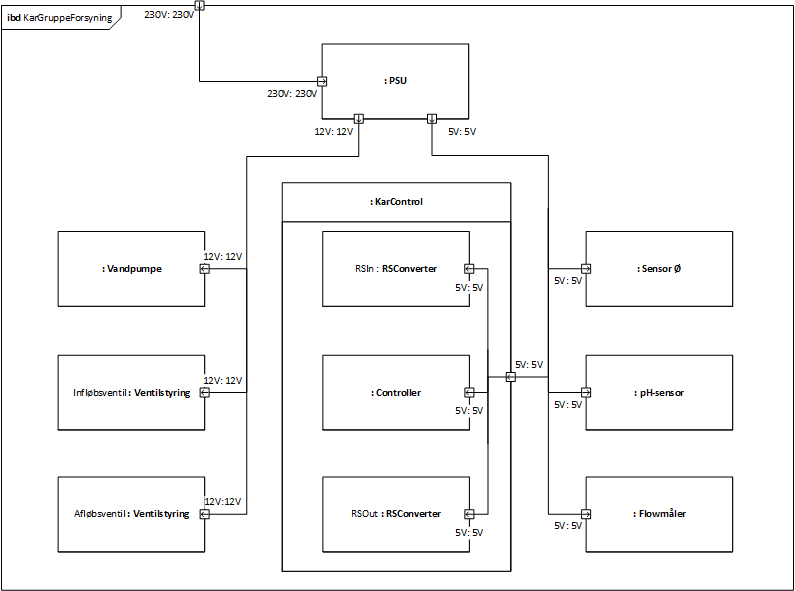
\includegraphics[scale=0.7]{Systemarkitektur/KarControl/KarControlForsyning_IBD.png}
	\label{fig:KarControlForsyning}
	\caption{IBD over forsyningsforbindelser til KarControl}
\end{figure}

%\subsection{KarControl Allokeringsdiagram}
%\systemAllokeringsDiagram{0.82}{KarControl}{KarControl}

\fxnote{Forsyningsspændinger skal have tolerancer}
\subsection{Signalbeskrivelser KarControl}
\systemSignaler{KarControl} {
KarBus				& RS485 bus til kommunikation mellem enheder &	 	& Differentielt bussystem  \\
OeBus				& RS485 bus til kommunikation mellem enheder &	 	& Differentielt bussystem  \\
Data485				& RS485 bus til kommunikation mellem enheder &	 	& internt signal   \\
Data232				& RS485 konverteret til logisk niveau		 &	 	& Signal efter konvertering  \\
EnableIndløb		& Signal til at lukke vand ind i kar		 & 0-5V	& Signal til at styre magnetventil   \\
EnableAfløb			& Signal til at lukke vand ud af kar		 & 0-5V	& Signal til at styre magnetventil	\\
EnableVandpumpe		& Signal til styring af vandpumpe			   	     & 0-5V & PWM styret signal	\\
Puls				& Takttæller af flow				   	 	 & 0-5V & 	\\
pH					& Analog signal fra pH måler			 	 & fra -420 til 420 mV  & Analogt signal	\\
Indløb				& vandstyring i kar							 &    	& Til at lukke vand ind i kar	\\
Afløb				& vandstyring i kar	 						 &   	& Til at lukke vand ud af kar	\\
Dossering			& vandstyring til planter					 &      & Til at dosere vand til planterne	\\
230V				& El-nettet som forsyner PSU				 & 230V	& \\
12V					& Forsyning til pumper og ventiler			 & 12V	& \\
5V					& Forsyning til systemets logiske kredsløb	 & 5V	& \\
}